\section{Entwurf}
\subsection{Schichtenarchitektur}
Die Anwendung wird in drei Schichten unterteilt, in aufsteigender Reihenfolge sind
dies die Datenabstraktionsschicht, die Anwendungslogikschicht und die Darstellungsschicht. Die
hierbei erkennbare Nähe zum ``Model View Controller''-Entwurfsmuster\footnote{siehe
\url{https://de.wikipedia.org/wiki/Model_View_Controller}} ist beabsichtigt und
im Hinblick auf die (hypothetische) nächste Ausbaustufe dieser Software --
nämlich den Schritt hin zu einer verteilten Multi-User-Anwendung, z.B. durch eine
über das Netzwerk angebundene, gemeinsam genutzte Datenbank -- sogar unerlässlich.

Jede Schicht abstrahiert ihre jeweilige Kernaufgabe von der nächsthöheren Schicht.
Abhängigkeiten sind jeweils nur unidirektional zwischen einer Schicht und
den darunterliegenden Schichten bzw. externen Bibliotheken erlaubt.

Eine Schicht kann -- z.B. zu Testzwecken -- komplett ausgetauscht werden; die
Schnittstelle zwischen den Schichten wird fest durch deren jeweilige Header-Files
definiert und ist unabhängig von der konkreten Implementierung. Eine
Schichtimplementierung darf insbesondere nicht Funktionalität, die über die
Standardschnittstelle hinaus geht, höheren Schichten zur Verfügung.

\subsubsection{Datenabstraktionsschicht}
\label{datenabstraktionsschicht}
Die Datenabstraktionsschicht stellt die unterste Schicht der Anwendung dar.
Ihre Aufgabe ist die Umsetzung einer prinzipiell format- und speichermedienunabhängigen
CRUD\footnote{Create, Read, Update, Delete}-Schittstelle, welche alle Datensätze
(und Operationen darauf) innerhalb einer Datenbank abbilden kann.

Hierzu gehören auch abstrakte Query-Operationen (prepared Statements), die im
einfachsten Fall schlicht an die zugrunde liegende SQL-Bibliothek weitergegeben
werden. Hierbei kommt in diesem Fall begünstigend hinzu, dass die vorliegende Datenbank
bisher ohnehin nur Integer, String und Blob-Werte erfasst, man also die Schnittstelle deutlich
vereinfachen kann.

Operationen der Datenabstraktionsschicht schreiben / lesen direkt (bzw. unerheblich
gepuffert) in die Datenbank. Hierbei ist auf Nichtverletzung des ACID-Prinzips\footnote{Siehe
\url{https://de.wikipedia.org/wiki/ACID}} zu achten --- dies wird insbesondere durch die Benutzung
von Transaktionen und -- in der Standardimplementierung -- durch das Verwenden von SQLite als
zugrundeliegende Datenbank erreicht.

\subsubsection{Anwendungslogikschicht}
Die Anwendungslogikschicht stellt der Darstellungsschicht auf hoher Abstraktionsebene Such-, Abfrage-
und Sortierfunktionen sowie Eingabevalidierung und einige Helferfunktionen, die von der Benutzeroberfläche
unabhängig sind (und bleiben sollen), zur Verfügung.

\subsubsection{Darstellungsschicht}
In der Darstellungsschicht werden schließlich Nutzereingaben entgegengenommen und
Datensätze wiedergegeben. Dies wird in diesem Fall wie gefordert über GTK+ umgesetzt,
kann aber theoretisch auch z.B. über ein via REST-API angebundenes HTML5-Frontend
realisiert werden.

Es ist möglich (und auch durchaus sinnvoll), die Anwendungslogikschicht als Bibliothek
aufzubauen und zu kompilieren, um dann verschiedenste Arten von Darstellungsschichten
nur noch gegen diese Bibliothek zu linken.

\subsection{Schnittstellenentwurf}
Ergebnis des Schnittstellenentwurfs sind die entsprechenden Header-Files der jeweiligen Module,
im Quellcodepaket im ordner \lstinline{include} auffindbar sind.

Aus der Schnittstellendokumentation, welche ebenda zu finden ist, ergeben sich auch Erklärungen zu
den Designentscheidungen, die während des Schnittstellenentwurfs getroffen wurden.
Ich verzichte an dieser Stelle auf eine Wiederholung dieser Schnittstellendokumentation und verweise
direkt auf die jeweiligen Header-Files.

Die Funktionen und Parameter zur Migration von Datenbanken sind in dieser ersten Version der Anwendung
vollkommen funktionslos. Dennoch müssen sie Teil einer gut geplanten Schnittstelle sein, um spätere
Änderungen am Datenformat zu ermöglichen, ohne die Kompatiblität der Kernbibliothek zu bereits existierender
Software verlieren.

\subsection{Datenbankentwurf}
Die relationale Datenbank, welche als Dateiformat auserkoren wurde, ist äußerst
einfach aufgebaut:

\begin{center}
\noindent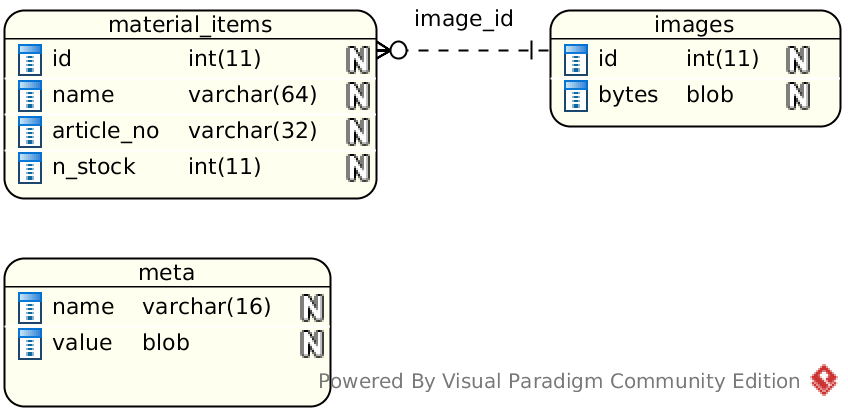
\includegraphics[width=110mm,keepaspectratio]{images/03-datenbankmodell.png}
\end{center}

Zusätzlich zum Domänenmodell ist hier lediglich die Tabelle ``meta'' neu: In ihr können
Konfigurations- und Metadaten aller Art gespeichert werden. Vorwiegend wird sie dafür
verwendet, die Version des Verwendeten Formats zu erfassen, sodass auch mit früheren
(oder späteren) Versionen der Anwendung erstellte Datenbanken verarbeitet werden können.
Die Inhalte dieser Tabelle werden nicht vollumfänglich über die Schnittstelle der
Datenabstraktionsschicht zur Verfügung gestellt bzw. veränderbar gemacht, können jedoch selektiv
und restriktiv zur Verfügung gestellt werden. (z.B. Datenbankversion als schreibgeschütztes Feld).

Der zum Aufbau dieser Datenbank erforderliche SQL-Code befindet sich bei den Quellcodes
zur Datenabstraktionsschicht.

\subsection{Anwendungsfälle und Screen Design}
Die Anwendungsfälle aus Benutzersicht wurden direkt via Glade in ein Screen Design umgesetzt, welches von der
Benutzerschnittstelle der Materialdatenbank eingelesen und direkt verwendet werden kann.

Im Folgenden findet sich eine Auflistung der erstellten Screen Designs sowie Randnotizen zu den damit verbundenen
Anwendungsfällen.

\subsubsection{Hauptfenster}
\begin{center}
\noindent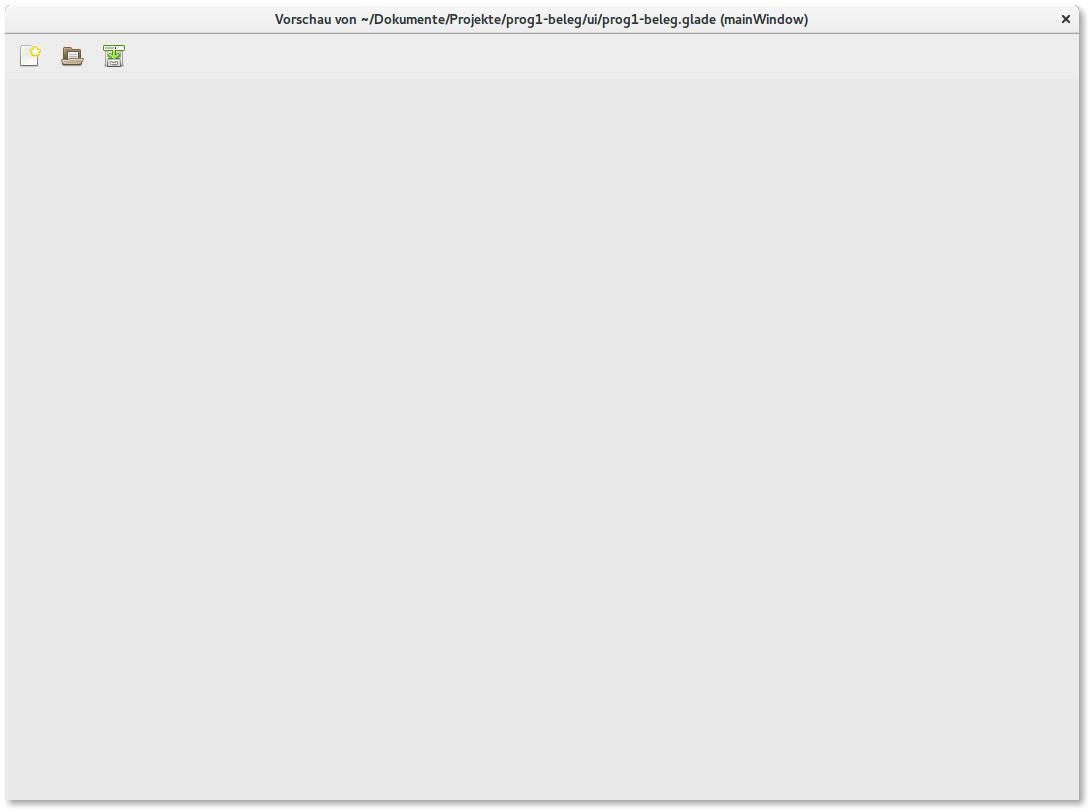
\includegraphics[width=150mm,keepaspectratio]{images/04-hauptfenster.png}
\end{center}

Das Hauptfenster stellt den äußeren Rahmen der Anwendung dar. Es ist bewusst minimalistisch aufgebaut, um vom eigentlichen
Inhalt der Anwendung nicht abzulenken, und besteht lediglich aus einer Werkzeugleiste für die Anwendungsfälle
``Neue Datenbank anlegen'', ``Bestehende Datenbank öffnen'' und ``Datenbank speichern unter'' sowie einer Statusleiste
für unkritische Systemmeldungen an den Benutzer.

Den Hauptteil des Fensters nehmen hingegen die jeweiligen Bildschirme ein, die im Folgenden aufgelistet sind.

\subsubsection{Willkommensbildschirm}
\begin{center}
\noindent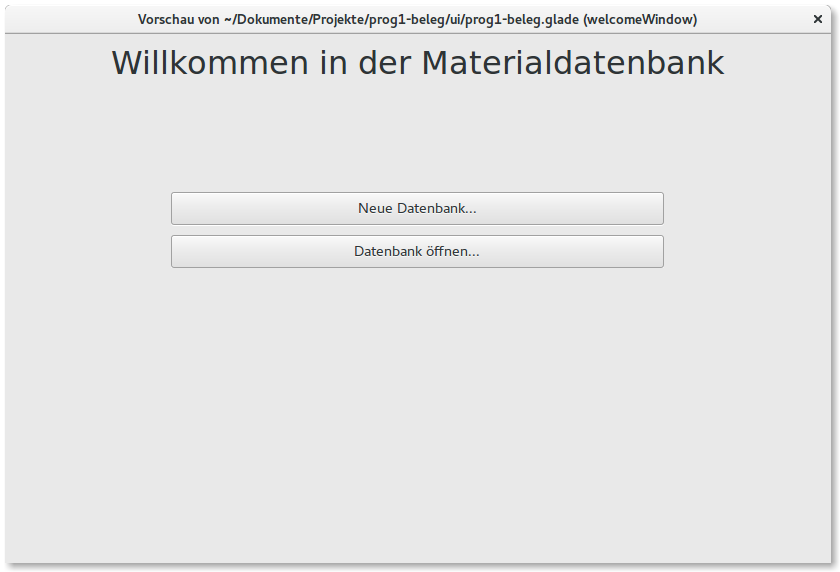
\includegraphics[width=150mm,keepaspectratio]{images/05-willkommensbildschirm.png}
\end{center}

Nach dem Starten der Anwendung wird dem Benutzer zunächst obiger Willkommensbildschirm präsentiert. Hier wird die
Aufmerksamkeit des Benutzers direkt auf die beiden wichtigsten Anwendungsfälle ``Neue Datenbank anlegen'' bzw.
``Bestehende Datenbank öffnen'' geleitet. Sinn und Zweck dieses Bildschirms ist es, gerade neuen Benutzern einen möglichst
einfachen Einstieg zu ermöglichen, aber auch das Steuerelement für das Öffnen einer bestehenden Datenbank zu spiegeln,
um bei wiederholtem Öffnen der Anwendung möglichst schnell weiter arbeiten zu können.

Eine naheliegende Erweiterung des Willkommensbildschirms wäre eine Liste zuletzt verwendeter Datenbanken, um nach dem
Öffnen der Anwendung möglichst mit einem Klick dort weiterzuarbeiten, wo der Benutzer zuvor aufgehört hatte.

Beim Erstellen des Screen Designs für den Willkommensbildschirm hat sich sehr schnell die mangelhafte Nutzerfreundlichkeit
und Stabilität\footnote{Es ist beispielsweise möglich, Glade mit dem versehentlichen Ablegen eines Widgets in sich
selbst unter bestimmen Voraussetzungen in eine Endlosschleife zu schicken, in welcher unkontrolliert Speicher allokiert
und somit das gesamte System blockiert wird. Diese Rekursion wäre eine leicht erkennbare Fehlerbedingung gewesen und hätte
durch achtsame Programmierung verhindert werden können. Als wäre dies nicht genug, gehen hierbei sogar trotz vorherigem
Speichervorgang Daten verloren -- unakzeptabel für eine Anwendung, die im professionellen Umfeld verwendet werden soll.}
von Glade gezeigt. Selbst das recht einfache Design des Willkommensbildschirms hat vergleichsweise viel
Zeit in Anspruch genommen, um mit Glade umgesetzt zu werden.
Hauptgründe hierfür sind die mangelhafte bzw. übereifrige Internationalisierung der Oberfläche von Glade\footnote{Auch geläufige
englische Fachbegriffe und Klassennamen wurden ``eingedeutscht'', was aber gerade für fortgeschrittene Entwickler
lediglich Verwirrung stiftet}, sowie mangelndes Feedback auf eine Vielzahl an Benutzereingaben, mangelnde Robustheit,
Intuitivität und Fehlertoleranz der Oberfläche.

Hier ist die Konkurrenz z.B. in Form des Frameworks Qt 5 und dessen Qt Designer oder Windows Forms / MFC in Kombination
mit Visual Studio dem GTK-Framework und Glade weit voraus.

Speziell für den Willkommensbildschirm war es leider nicht möglich, die Buttons mit Icons auszustatten, ohne sie von ihrer
zugewiesenen GTK-Aktion zu trennen.